\begin{enumerate}
	\item{
	% Part a
		Convert circtuit to its s domain equivalent:
		\begin{figure}[H]
			\centering
			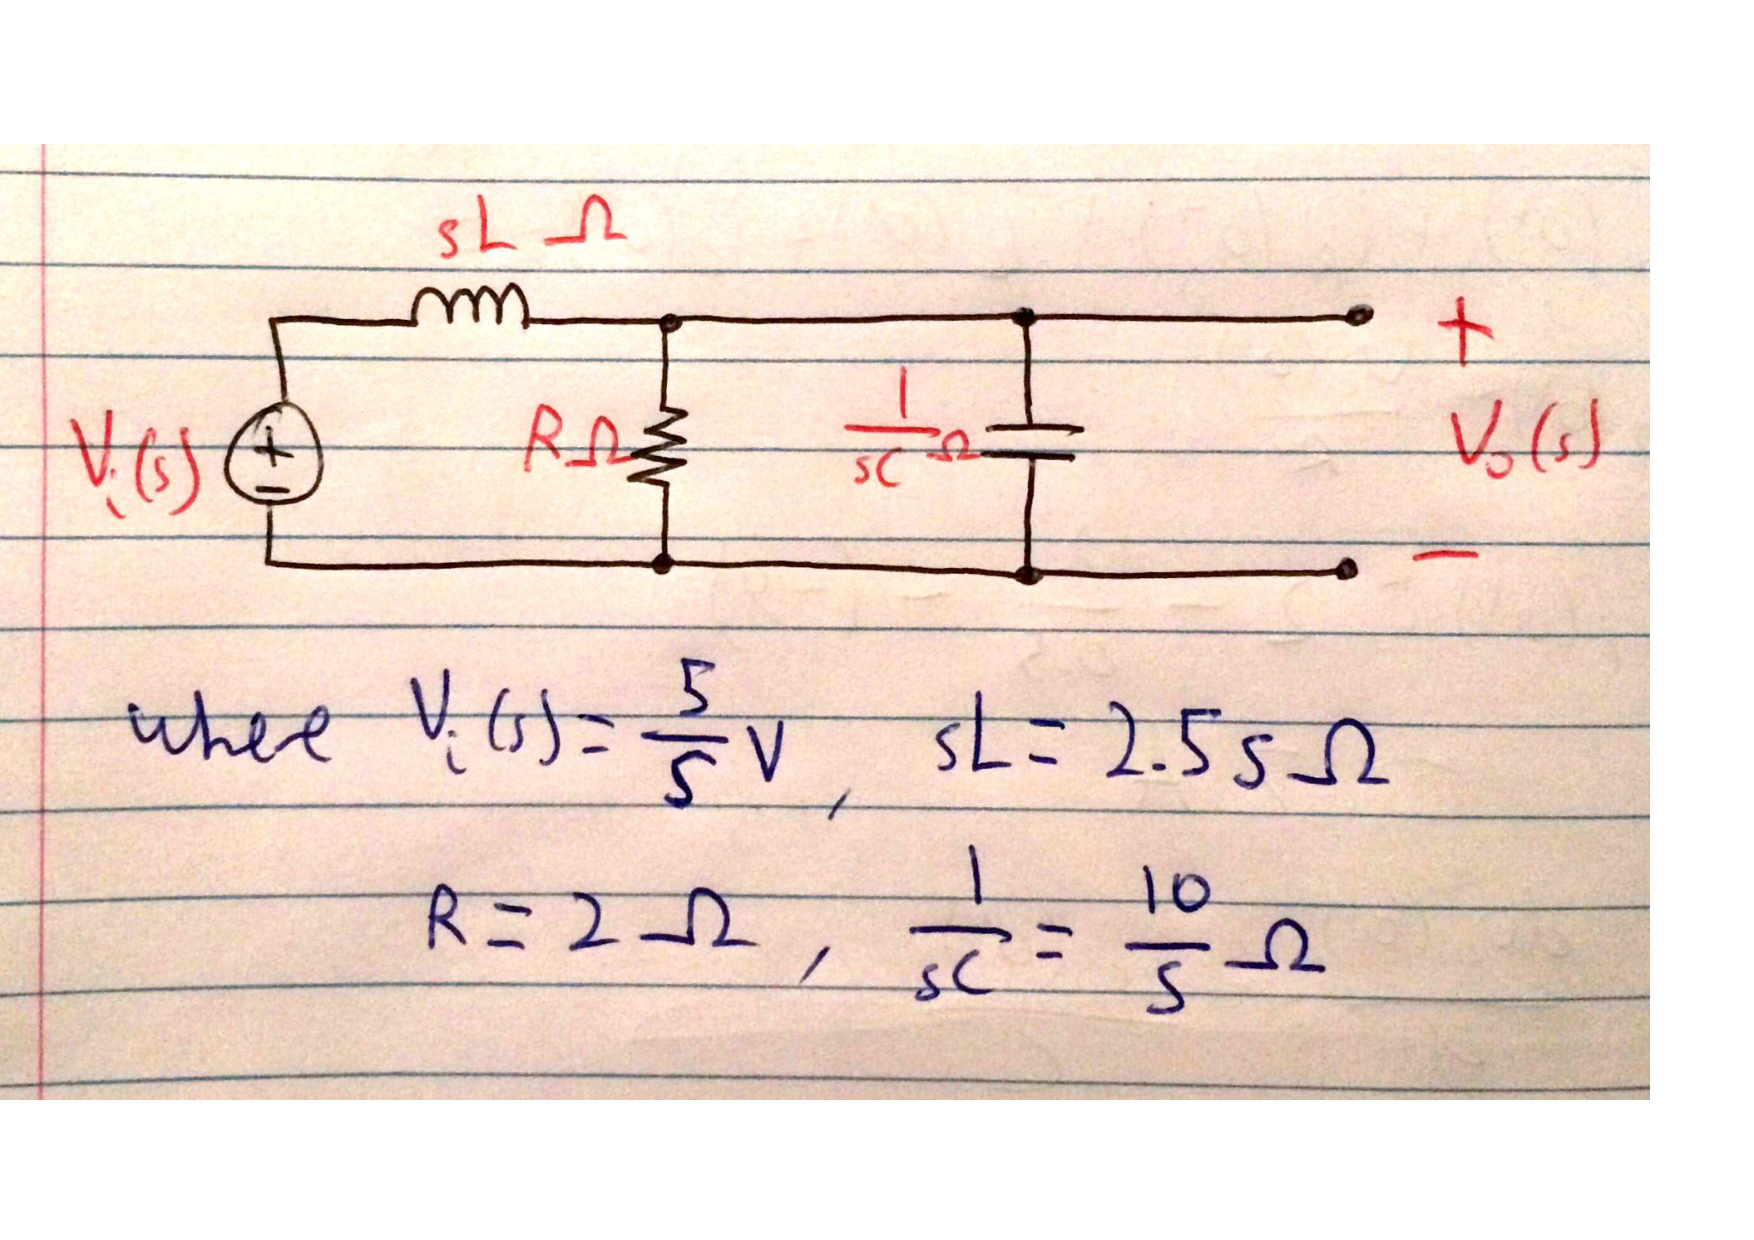
\includegraphics[scale=0.55]{q2a.pdf}
		\end{figure}
		The circuit is a voltage divider:
		\begin{align*}
			V_o(s) &= V_i(s) \times \frac{Z_R || Z_C}{Z_R || Z_C + Z_L} \\
			&= \frac{5}{s} \times \frac{\frac{20s}{s(2s+10)}}{\frac{20s}{s(2s+10)}+2.5s} \\
			&= \frac{5}{s} \times \frac{1}{1+0.125(2s^2+10s)} \\
			&= \frac{5}{s(0.25s^2+1.25s+1)} \\
			&= \frac{20}{s(s+4)(s+1)}
		\end{align*}
		Perform partial fraction expansion:
		\begin{equation*}
			\frac{20}{s(s+4)(s+1)} = \frac{A}{s} + \frac{B}{s+4} + \frac{C}{s+1}
		\end{equation*}
		\begin{equation*}
			\therefore 20 = A(s+4)(s+1) + Bs(s+1) + Cs(s+4)
		\end{equation*}
		Now solve for A, B and C:
		\begin{equation*}
			s = 0 \implies 20 = A(4)(1) \implies A = 5
		\end{equation*}
		\begin{equation*}
			s = -4 \implies 20 = B(-4)(-3) \implies B = \frac{5}{3}
		\end{equation*}
		\begin{equation*}
			s = -1 \implies 20 = C(-1)(3) \implies C = -\frac{20}{3}
		\end{equation*}
		And we arrive at $V_o(s)$ in partial fraction expanded form:
		\begin{equation*}
			V_o(s) = \frac{5}{s} + \frac{5}{3(s+4)} - \frac{20}{3(s+1)} \ \mathrm{V}
		\end{equation*}
		\\
	}

	\item{
	%Part b
		Perform the inverse Laplace transform:
		\begin{align*}
			v_o(t) &= \mathcal{L}^{-1}\left[ V_o(s) \right] \\
			&= \left(5 + \frac{5}{3}e^{-4t} - \frac{20}{3}e^{-t} \right) u(t) \ \mathrm{V}
		\end{align*}
		\\
	}

	\item{
	%Part c
		The circuit elements (R, L and C) remain the same, therefore $s_1, s_2$ and the form of equation will remain the same. 
		\par
		Input voltage source (forcing function) remains the same, therefore the steady state component of response will remain the same.
		\par
		One or both of the coefficients of the transient component terms may change, as these are the only parts of the response equation that are determined by the initial conditions.
		\\
	}

\end{enumerate}
